\documentclass[tikz, preview]{standalone}
\usepackage{amsfonts, amsthm, amssymb, amsmath, stmaryrd, etoolbox}
\usepackage{tikz}
\usetikzlibrary{matrix,arrows}
\newcommand{\A}{\mathbf{A}}
\newcommand{\X}{\mathbf{X}}
\begin{document}
%%%%%%%%%%%%%%%%%	
%%%%%%%%%%%%%%%%%
\[
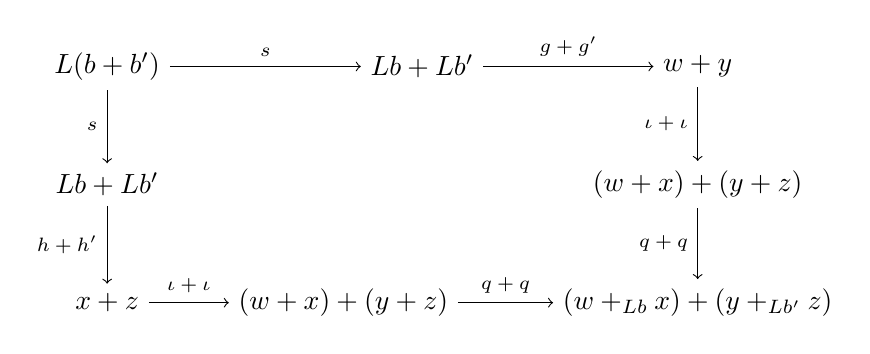
\begin{tikzpicture}
%	\draw [help lines, step=0.5, color=blue!10] (-1,-5) grid (10,5); % grid
	% corner nodes
	\node (dom) at (0,3) {$ L ( b + b' ) $};
	\node (cod) at (7.5,0) {$ ( w +_{ Lb } x ) + ( y +_{ Lb' } z ) $};
	% top path nodes
	\node (t1) at (4,3) {$ Lb + Lb' $};
	\node (t2) at (7.5,3) {$ w + y $};
	\node (t3) at (7.5,1.5) {$ ( w + x ) + ( y + z ) $};
	% bottom path nodes
	\node (b1) at (0,1.5) {$ Lb + Lb' $};
	\node (b2) at (0,0) {$ x + z $};
	\node (b3) at (3,0) {$ ( w + x ) + ( y + z ) $};
	%
	% top path arrows
	\draw [->] (dom) to node [above] {\scriptsize $ s $} (t1);
	\draw [->] (t1) to node [above] {\scriptsize $ g + g' $} (t2);
	\draw [->] (t2) to node [left] {\scriptsize $ \iota + \iota $} (t3);
	\draw [->] (t3) to node [left] {\scriptsize $ q + q $} (cod);
	% bottom path arrows
	\draw [->] (dom) to node [left] {\scriptsize $ s $} (b1);
	\draw [->] (b1) to node [left] {\scriptsize $ h + h' $} (b2);
	\draw [->] (b2) to node [above] {\scriptsize $ \iota + \iota $} (b3);
	\draw [->] (b3) to node [above] {\scriptsize $ q + q $} (cod);
\end{tikzpicture}
\]
%%%%%%%%%%%%%%%%%
%%%%%%%%%%%%%%%%%
\end{document}
